\RequirePackage{atbegshi}
\documentclass[compress,aspectratio=169]{beamer}\usepackage[]{graphicx}\usepackage[]{xcolor}
% maxwidth is the original width if it is less than linewidth
% otherwise use linewidth (to make sure the graphics do not exceed the margin)
\makeatletter
\def\maxwidth{ %
  \ifdim\Gin@nat@width>\linewidth
    \linewidth
  \else
    \Gin@nat@width
  \fi
}
\makeatother

\definecolor{fgcolor}{rgb}{0.345, 0.345, 0.345}
\newcommand{\hlnum}[1]{\textcolor[rgb]{0.686,0.059,0.569}{#1}}%
\newcommand{\hlstr}[1]{\textcolor[rgb]{0.192,0.494,0.8}{#1}}%
\newcommand{\hlcom}[1]{\textcolor[rgb]{0.678,0.584,0.686}{\textit{#1}}}%
\newcommand{\hlopt}[1]{\textcolor[rgb]{0,0,0}{#1}}%
\newcommand{\hlstd}[1]{\textcolor[rgb]{0.345,0.345,0.345}{#1}}%
\newcommand{\hlkwa}[1]{\textcolor[rgb]{0.161,0.373,0.58}{\textbf{#1}}}%
\newcommand{\hlkwb}[1]{\textcolor[rgb]{0.69,0.353,0.396}{#1}}%
\newcommand{\hlkwc}[1]{\textcolor[rgb]{0.333,0.667,0.333}{#1}}%
\newcommand{\hlkwd}[1]{\textcolor[rgb]{0.737,0.353,0.396}{\textbf{#1}}}%
\let\hlipl\hlkwb

\usepackage{framed}
\makeatletter
\newenvironment{kframe}{%
 \def\at@end@of@kframe{}%
 \ifinner\ifhmode%
  \def\at@end@of@kframe{\end{minipage}}%
  \begin{minipage}{\columnwidth}%
 \fi\fi%
 \def\FrameCommand##1{\hskip\@totalleftmargin \hskip-\fboxsep
 \colorbox{shadecolor}{##1}\hskip-\fboxsep
     % There is no \\@totalrightmargin, so:
     \hskip-\linewidth \hskip-\@totalleftmargin \hskip\columnwidth}%
 \MakeFramed {\advance\hsize-\width
   \@totalleftmargin\z@ \linewidth\hsize
   \@setminipage}}%
 {\par\unskip\endMakeFramed%
 \at@end@of@kframe}
\makeatother

\definecolor{shadecolor}{rgb}{.97, .97, .97}
\definecolor{messagecolor}{rgb}{0, 0, 0}
\definecolor{warningcolor}{rgb}{1, 0, 1}
\definecolor{errorcolor}{rgb}{1, 0, 0}
\newenvironment{knitrout}{}{} % an empty environment to be redefined in TeX

\usepackage{alltt} % aspectratio=169


% % % % % % % % % % % % % % %
%             MY PACKAGES 
% % % % % % % % % % % % % % %
\usepackage{graphicx}       % Use pdf, png, jpg, or eps with pdflatex; use eps in DVI mode
\usepackage{dcolumn} % this pack is neccesary to build nicer columns with texreg--dont remove it.
\usepackage[export]{adjustbox}
\usepackage{xcolor}[dvipsnames]
\usepackage{amssymb,amsmath}
\usepackage{threeparttable} % package to have long notes in reg tables in texreg. 
\usepackage{graphics}
\usepackage{pgfplots}
\pgfplotsset{compat=1.11}
\usepgfplotslibrary{fillbetween}
\usepackage{fontawesome}


%\usepackage{tipx}
%\usepackage{tikz}
%\usetikzlibrary{arrows,shapes,decorations.pathmorphing,backgrounds,positioning,fit,petri}
\usepackage{rotating}
%\usepackage{scalerel} % for inline images
\usepackage{import}
%\usepackage{times}
\usepackage{array}
\usepackage{tabularx}
\usepackage{booktabs}
%\usepackage{textcomp}
\usepackage{float}
%\usepackage{setspace}      % \doublespacing \singlespacing \onehalfspacing %doble espacio
%\label{x:y}                          %ocupar para autoref.
%\autoref{x:y}                        %ocupar para autoref.
%\usepackage{nopageno}      %desactivar para p�ginas
\usepackage{pifont}
\newcommand{\xmark}{\ding{55}}%

%\usepackage{marvosym} %faces

\usepackage{hyperref}
\hypersetup{
    %bookmarks=true,         % show bookmarks bar?
    unicode=false,          % non-Latin characters in Acrobat’s bookmarks
    pdftoolbar=true,        % show Acrobat’s toolbar?
    pdfmenubar=true,        % show Acrobat’s menu?
    pdffitwindow=true,     % window fit to page when opened
    pdfstartview={FitH},    % fits the width of the page to the window
    pdftitle={My title},    % title
    pdfauthor={Author},     % author
    pdfsubject={Subject},   % subject of the document
    pdfcreator={Creator},   % creator of the document
    pdfproducer={Producer}, % producer of the document
    pdfkeywords={keyword1} {key2} {key3}, % list of keywords
    pdfnewwindow=true,      % links in new window
    colorlinks=true,       % false: boxed links; true: colored links
    linkcolor=blue,          % color of internal links (change box color with linkbordercolor)
    citecolor=blue,        % color of links to bibliography
    filecolor=blue,      % color of file links
    urlcolor=blue           % color of external links
}

\hypersetup{
  colorlinks = true,
  urlcolor = blue,
  pdfpagemode = UseNone
}


\usepackage{multirow}

\usepackage{tikz}
\usetikzlibrary{arrows,decorations.pathreplacing}



\usepackage{listings}
\usepackage{color}
\definecolor{dkgreen}{rgb}{0,0.6,0}
\definecolor{gray}{rgb}{0.5,0.5,0.5}
\definecolor{mauve}{rgb}{0.58,0,0.82}
\lstset{ %
  language=R,                     % the language of the code
  basicstyle=\TINY,           % the size of the fonts that are used for the code
  numbers=left,                   % where to put the line-numbers
  numberstyle=\tiny\color{gray},  % the style that is used for the line-numbers
  stepnumber=1,                   % the step between two line-numbers. If it's 1, each line
                                  % will be numbered
  numbersep=5pt,                  % how far the line-numbers are from the code
  backgroundcolor=\color{white},  % choose the background color. You must add \usepackage{color}
  showspaces=false,               % show spaces adding particular underscores
  showstringspaces=false,         % underline spaces within strings
  showtabs=false,                 % show tabs within strings adding particular underscores
  frame=single,                   % adds a frame around the code
  rulecolor=\color{black},        % if not set, the frame-color may be changed on line-breaks within not-black text (e.g. commens (green here))
  tabsize=1,                      % sets default tabsize to 2 spaces
  captionpos=b,                   % sets the caption-position to bottom
  breaklines=true,                % sets automatic line breaking
  breakatwhitespace=false,        % sets if automatic breaks should only happen at whitespace
  title=\lstname,                 % show the filename of files included with \lstinputlisting;
                                  % also try caption instead of title
  keywordstyle=\color{blue},      % keyword style
  commentstyle=\color{dkgreen},   % comment style
  stringstyle=\color{mauve},      % string literal style
  escapeinside={\%*}{*)},         % if you want to add a comment within your code
  morekeywords={*,...}            % if you want to add more keywords to the set
} 

% % % % % % % % % % % % % % %
%           PACKAGE CUSTOMIZATION
% % % % % % % % % % % % % % %

% GENERAL CUSTOMIZATION
\usepackage[math]{iwona}% font
\usetheme{Singapore}  % template I should use
%\usetheme{Szeged}  % alternative template
\usecolortheme{rose}  % color template
\makeatletter     % to show subsection/section title (1/3)
\beamer@theme@subsectiontrue % to show subsection/section title (2/3)
\makeatother      % to show subsection/section title (3/3)



% THIS BELOW IS TO MAKE NAVIGATION DOTS MARKED DURING PRESENTATION
\makeatletter
\def\slideentry#1#2#3#4#5#6{%
  %section number, subsection number, slide number, first/last frame, page number, part number
  \ifnum#6=\c@part\ifnum#2>0\ifnum#3>0%
    \ifbeamer@compress%
      \advance\beamer@xpos by1\relax%
    \else%
      \beamer@xpos=#3\relax%
      \beamer@ypos=#2\relax%
    \fi%
  \hbox to 0pt{%
    \beamer@tempdim=-\beamer@vboxoffset%
    \advance\beamer@tempdim by-\beamer@boxsize%
    \multiply\beamer@tempdim by\beamer@ypos%
    \advance\beamer@tempdim by -.05cm%
    \raise\beamer@tempdim\hbox{%
      \beamer@tempdim=\beamer@boxsize%
      \multiply\beamer@tempdim by\beamer@xpos%
      \advance\beamer@tempdim by -\beamer@boxsize%
      \advance\beamer@tempdim by 1pt%
      \kern\beamer@tempdim
      \global\beamer@section@min@dim\beamer@tempdim
      \hbox{\beamer@link(#4){%
          \usebeamerfont{mini frame}%
          \ifnum\c@section>#1%
            %\usebeamercolor[fg]{mini frame}%
            %\usebeamertemplate{mini frame}%
            \usebeamercolor{mini frame}%
            \usebeamertemplate{mini frame in other subsection}%
          \else%
            \ifnum\c@section=#1%
              \ifnum\c@subsection>#2%
                \usebeamercolor[fg]{mini frame}%
                \usebeamertemplate{mini frame}%
              \else%
                \ifnum\c@subsection=#2%
                  \usebeamercolor[fg]{mini frame}%
                  \ifnum\c@subsectionslide<#3%
                    \usebeamertemplate{mini frame in current subsection}%
                  \else%
                    \usebeamertemplate{mini frame}%
                  \fi%
                \else%
                  \usebeamercolor{mini frame}%
                  \usebeamertemplate{mini frame in other subsection}%
                \fi%
              \fi%
            \else%
              \usebeamercolor{mini frame}%
              \usebeamertemplate{mini frame in other subsection}%
            \fi%
          \fi%
        }}}\hskip-10cm plus 1fil%
  }\fi\fi%
  \else%
  \fakeslideentry{#1}{#2}{#3}{#4}{#5}{#6}%
  \fi\ignorespaces
  }
\makeatother


%%% bib begin
\usepackage[authordate,isbn=false,doi=false,url=false,eprint=false]{biblatex-chicago}
\DeclareFieldFormat[article]{title}{\mkbibquote{#1}} % make article titles in quotes
\DeclareFieldFormat[thesis]{title}{\mkbibemph{#1}} % make theses italics

\AtEveryBibitem{\clearfield{month}}
\AtEveryCitekey{\clearfield{month}}

\addbibresource{/Users/hectorbahamonde/Bibliografia_PoliSci/library.bib} 


% USAGES
%% use \textcite to cite normal
%% \parencite to cite in parentheses
%% \footcite to cite in footnote
%% the default can be modified in autocite=FOO, footnote, for ex. 
%%% bib end



% % % % % % % % % % % % % % %
%       To show the TITLE at the Bottom of each slide
% % % % % % % % % % % % % % %

\beamertemplatenavigationsymbolsempty 
\makeatletter
\setbeamertemplate{footline}
{
\leavevmode%
\hbox{%
\begin{beamercolorbox}[wd=1\paperwidth,ht=2.25ex,dp=2ex,center]{title in head/foot}%
\usebeamerfont{title in head/foot}\insertshorttitle
\end{beamercolorbox}%
\begin{beamercolorbox}[wd=1
\paperwidth,ht=2.25ex,dp=2ex,center]{date in head/foot}%
\end{beamercolorbox}}%
}
\makeatother



% to switch off navigation bullets
%% using \miniframeson or \miniframesoff
\makeatletter
\let\beamer@writeslidentry@miniframeson=\beamer@writeslidentry
\def\beamer@writeslidentry@miniframesoff{%
  \expandafter\beamer@ifempty\expandafter{\beamer@framestartpage}{}% does not happen normally
  {%else
    % removed \addtocontents commands
    \clearpage\beamer@notesactions%
  }
}
\newcommand*{\miniframeson}{\let\beamer@writeslidentry=\beamer@writeslidentry@miniframeson}
\newcommand*{\miniframesoff}{\let\beamer@writeslidentry=\beamer@writeslidentry@miniframesoff}
\makeatother

% Image full size: use 
%%\begin{frame}
  %%\fullsizegraphic{monogram.jpg}
%%\end{frame}
\newcommand<>{\fullsizegraphic}[1]{
  \begin{textblock*}{0cm}(-1cm,-3.78cm)
  \includegraphics[width=\paperwidth]{#1}
  \end{textblock*}
}


% hyperlinks
\hypersetup{colorlinks,
            urlcolor=[rgb]{0.01, 0.28, 1.0},
            linkcolor=[rgb]{0.01, 0.28, 1.0}}



%\newcommand{\vitem}[]{\vfill \item}

% % % % % % % % % % % % % % %
%           DOCUMENT ID
% % % % % % % % % % % % % % %

\title{\input{title.txt}\unskip} % 




\author[shortname]{
Hector Bahamonde \inst{1} \and 
Inga Saikkonen \inst{2} \and 
Mart Trasberg \inst{3} \\ \vspace{3mm} \scriptsize{\color{gray}Authors in alphabetical order. All contributed equally to this project.}
}

\institute[shortinst]{\inst{1} University of Turku, Finland \and %
                      \inst{2} \textnormal{Åbo Akademi}, Finland \and
                      \inst{3} Monterrey Tec, Mexico}







\date{\today}

%to to see shadows of previous blocks
%\setbeamercovered{dynamic}
\IfFileExists{upquote.sty}{\usepackage{upquote}}{}
\begin{document}

















% % % % % % % % % % % % % % %
%           CONTENT
% % % % % % % % % % % % % % %

%% title frame
\begin{frame}
\titlepage
\end{frame}


\section{Introduction}


\subsection{Motivation}

\miniframeson
\begin{frame}[c]{Democratic Backsliding}
  \begin{itemize}
    \item Parece existir un consenso en que algunas democracias est\'an en riesgo de retroceder (\emph{democratic backsliding}).

    \item Estos retrocesos han sido estudiados en un sinn\'umero de casos.

        \begin{itemize}
          \item \textcite{Kaufman2019} explican que ``a transition to competitive authoritarianism in the United States is unlikely, although not impossible.''

          \item {\bf {\color{red}Caso 2}.}
          \item {\bf {\color{red}Caso 3}.}

        \end{itemize}

  \end{itemize}
\end{frame} 

\miniframesoff
\begin{frame}[c]{Democratic Backsliding: A ``Winners Bias''}

Desafortunadamente, la major\'ia ha concentrado sus esfuerzos en c\'omo el {\bf ejecutivo} \emph{agranda} sus poderes. 

    \begin{itemize}
      \item \textcite[p. 27]{Haggard2021} definen ``[d]emocratic backsliding is the incremental erosion of institutions [...] that results from the actions of [...] {\bf \emph{elected} governments}.''

      \item \textcite[p. 2]{Perez-Linan2018} explica que ``most threats to democracy originate in the {\bf \emph{executive}}, not in congress.''

      \item \textcite[p. 41]{Corrales2020} explica que ``electoral irregularities contributed to democratic backsliding in Venezuela under {\bf \emph{chavista} rule}.''

    \end{itemize}

\begin{alertblock}{What about the \underline{electoral lossers}?}
Qu\'e ocurre con los que pierden la elecci\'on? Existen diferencias sistem\'aticas en cuanto la tolerancia de acciones no democr\'aticas entre ``ganadores'' y ``perdedores''?
\end{alertblock}
    
\end{frame}

\subsection{Our Paper}

\miniframeson
\begin{frame}[c]{Nuestro Paper: ``El baile de los que sobran''}

  \begin{itemize}
    \item A diferencia de la mayoría de quienes estudian posibles violaciones de los principios democr\'aticos por parte de los ``ganadores,'' nosotros estudiamos a los ``{\bf perdedores}'' electorales.

    \item Hicimos un survey experiment (pre-registrado) en dos democracias recientes, Chile (y Estonia).

    \item {\color{blue} Entender si los votantes que apoyaron al {\bf candidato perdedor} est\'an más abiertos a respaldar acciones anti-sist\'emicas {\bf contra el ganador}}.

    \item Para esto, incluimos una teor\'ia enfocada en \emph{pérdidas} y \emph{loss aversion} (``\emph{prospect theory},'' e.g., \cite{Kahneman1979}).

    %\item {\bf Pre-registered findings}: encontramos que los votantes de {\bf Kast} \emph{no} son mas proclives que los votantes de {\bf Boric} a apoyar acciones antisist\'emicas (protestas). 

  \end{itemize}

      \begin{exampleblock}{Findings} 
      Encontramos que los votantes de {\bf Kast} \emph{no} son mas proclives que los votantes de {\bf Boric} a apoyar acciones antisist\'emicas (protestas) que pongan en peligro el status quo. 
      \end{exampleblock}
  
\end{frame}


\section{Theory}

\subsection{Democratic Backsliding}

\miniframeson
\begin{frame}[c]{Democratic Backsliding}

  \begin{itemize}
    \item Test
  \end{itemize}

\end{frame}

\subsection{Prospect Theory}



\miniframeson
\begin{frame}[c]{Prospect Theory}

  \begin{itemize}

    \item {\bf Losses loom larger than gains}: individuals ``give more weight to losses than to comparable gains'' \scriptsize{\parencite[p. 171]{Levy1992a}}.

    \normalsize{\item{\bf Loss aversion}: individuals ``are more concerned with preventing a decline than increasing gains'' \scriptsize{\parencite[p. 89]{Levy1997}}}.
    
    %\item Utilities are defined with regard to \emph{changes} in outcomes with respect to a reference point.
    
    \item {\bf Asymmetric decision making}: ``[I]ndividuals tend to be risk averse in a domain of gains, and relatively risk seeking in a domain of losses'' \scriptsize{\parencite[p. 18]{McDermott1998}}.
    
  \end{itemize}

\end{frame}


\section{Argument}

\subsection{Argument}

\miniframeson
\begin{frame}[c]{Pre-Registered Hypothesis}

\begin{exampleblock}{Argument}
Respondents who voted for the candidate/party that lost the the last election (Kast) would be more likely to choose a candidate who supports anti-systemic actions (protests) against the current government than respondents in the ``winning side.'' 
\end{exampleblock}

\end{frame}


\section{Empirics}

\subsection{Experimental Design}

\miniframeson
\begin{frame}[c]{Conjoint Experiment}

  \begin{itemize}
    \item Disenamos un conjoint experiment {\scriptsize\parencite{Hainmueller2014}}.
    \item La muestra es representativa a nivel pais ($n=741$).
    \item Fully randomized design (no constrains).
    \item Representatividad estad\'istica de g\'enero y partido.
    \item Bater\'ia de socio-demogr\'aficos, intenci\'on pol\'itica (Kast, Boric), evaluaci\'on de la democracia.
  \end{itemize}

\begin{table}[h]
%\begin{footnotesize}
\scalebox{0.7}{
\begin{tabular}{  c |  p{0.6\linewidth} }
\toprule
\textbf{Dimension} & \textbf{Attribute Set} \\
\midrule
{\only<1,2>{\leavevmode\color{blue}}Gender} & {\only<1>{\leavevmode\color{red}}Male}, {\only<2>{\leavevmode\color{red}}Female}. \\
{\only<3,4,5>{\leavevmode\color{blue}}Age} & {\only<3>{\leavevmode\color{red}}Younger than 35}, {\only<4>{\leavevmode\color{red}}Between 35-50}, {\only<5>{\leavevmode\color{red}}Over 50}. \\
{\only<6,7>{\leavevmode\color{blue}}Protest} & {\only<6>{\leavevmode\color{red}}The candidate OPPOSES anti-government protest that will seek to de-destabilize the current government}, {\only<7>{\leavevmode\color{red}}The candidate SUPPORTS anti-government protest that will seek to de-destabilize the current government} \\
\bottomrule
\end{tabular}}
%\end{footnotesize}
\end{table}
\end{frame}




\subsection{Statistical Analyses}


\miniframeson
\begin{frame}[c]{Subgroup Marginal Means (MM)}

  \begin{itemize}
    \item We depart from standard AMCE analyses {\scriptsize\parencite{Hainmueller2014}} and instead compute {\bf subgroup marginal means} {\scriptsize\parencite{Leeper2020a}}.
    \item In practice, when using marginal means, there's no need to set a reference category.
    \item ``In a forced-choice conjoint design, the grand mean is by definition 0.5'' {\scriptsize\parencite[p. 209]{Leeper2020a}}.
  \end{itemize}

\end{frame}



\subsection{Results}


\miniframeson
\begin{frame}[c]{Subgroup Marginal Means (MM): Boric, Kast}

\begin{center}
          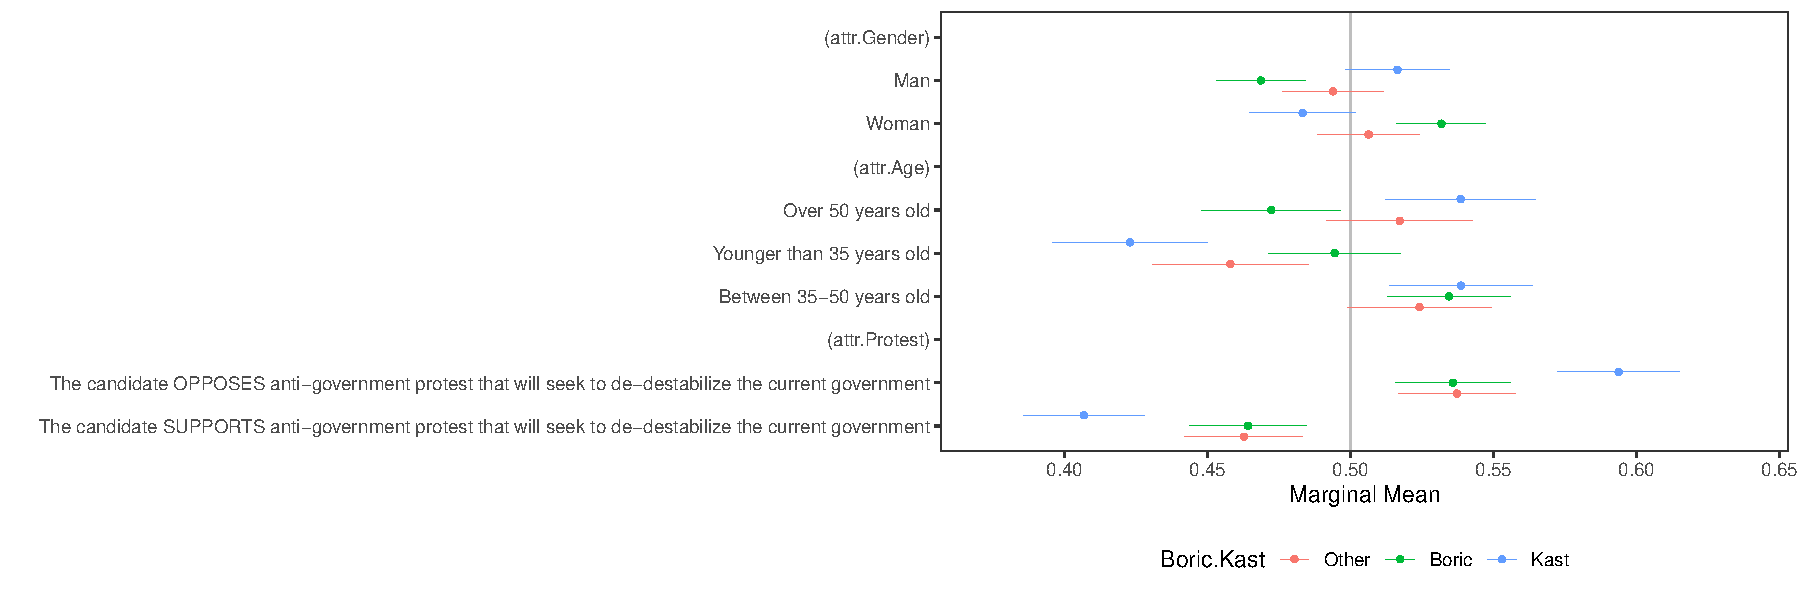
\includegraphics[scale=0.5, center]{/Users/hectorbahamonde/research/democratic_backsliding/Boric_Kast.pdf}
\end{center}
\end{frame}

%\miniframesoff
%\begin{frame}[c]{Other Descriptive Results: Support for Democracy}
%
%\begin{center}
%          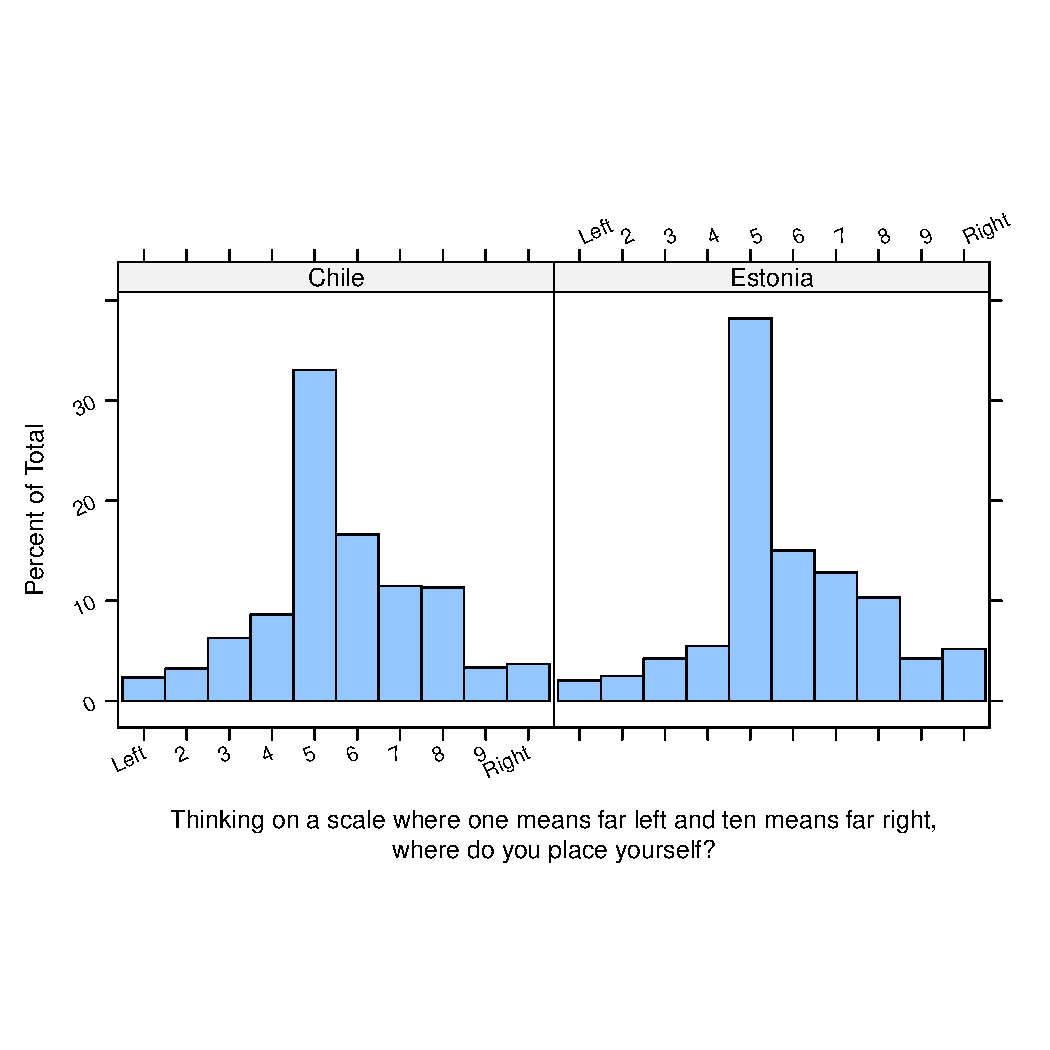
\includegraphics[scale=0.65, center]{/Users/hectorbahamonde/research/democratic_backsliding/left_right.pdf}
%\end{center}
%\end{frame}

\subsection{Descriptive Results}


\miniframeson
\begin{frame}[c]{Other Descriptive Results: Support for Democracy}

\begin{center}
          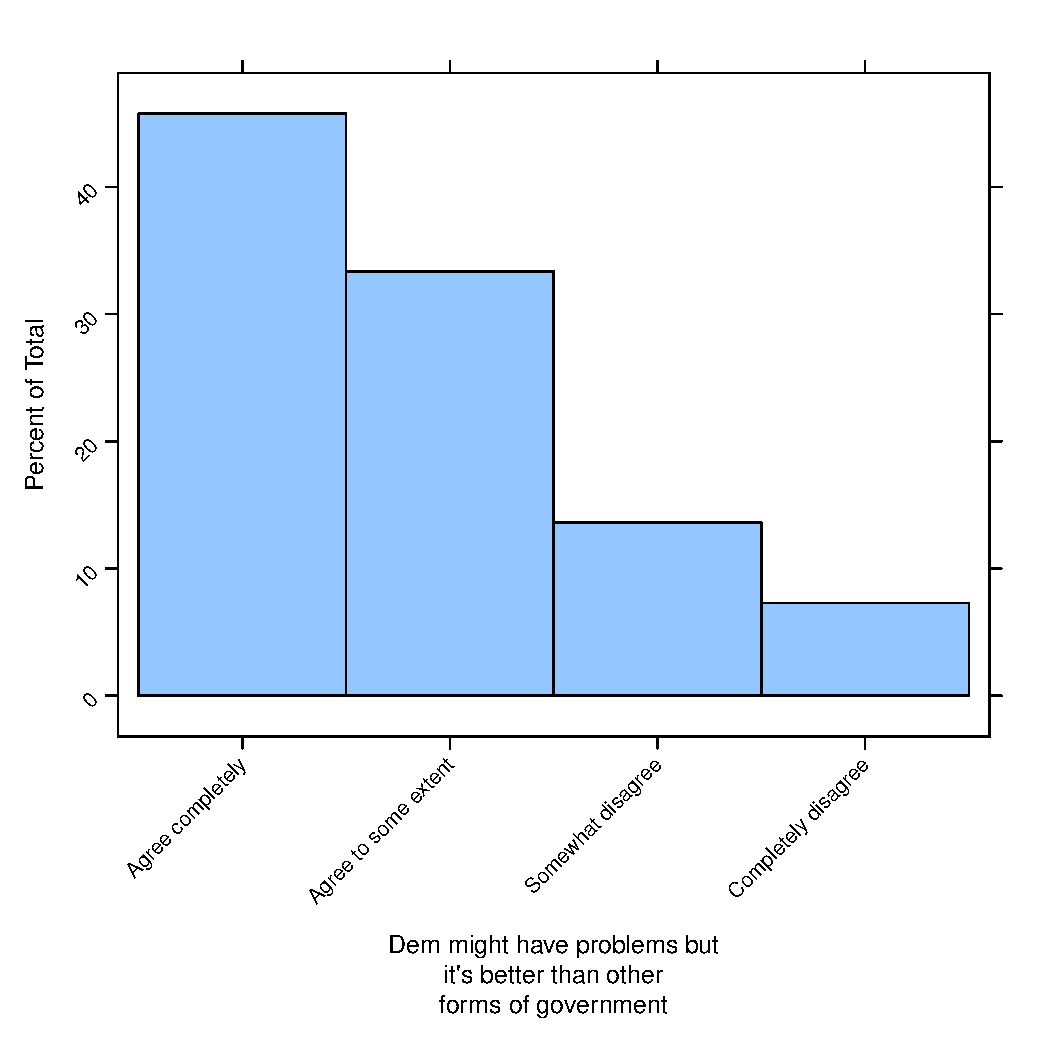
\includegraphics[scale=0.35, center]{/Users/hectorbahamonde/research/democratic_backsliding/dem_better.pdf}
\end{center}
\end{frame}

\miniframesoff
\begin{frame}[c]{Other Descriptive Results: Support for Democracy}

\begin{center}
          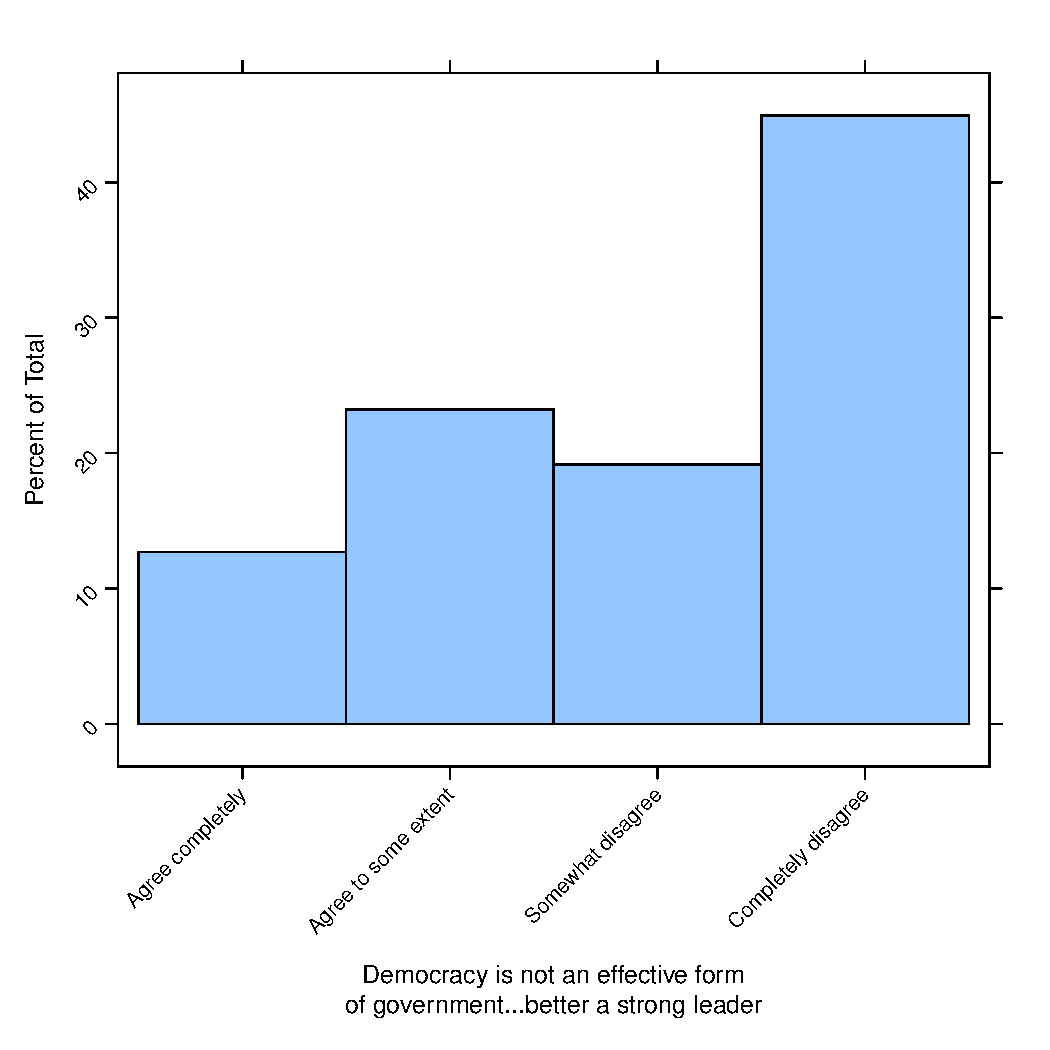
\includegraphics[scale=0.35, center]{/Users/hectorbahamonde/research/democratic_backsliding/strong_leader.pdf}
\end{center}
\end{frame}

\miniframesoff
\begin{frame}[c]{Other Descriptive Results: Support for Democracy}

\begin{center}
          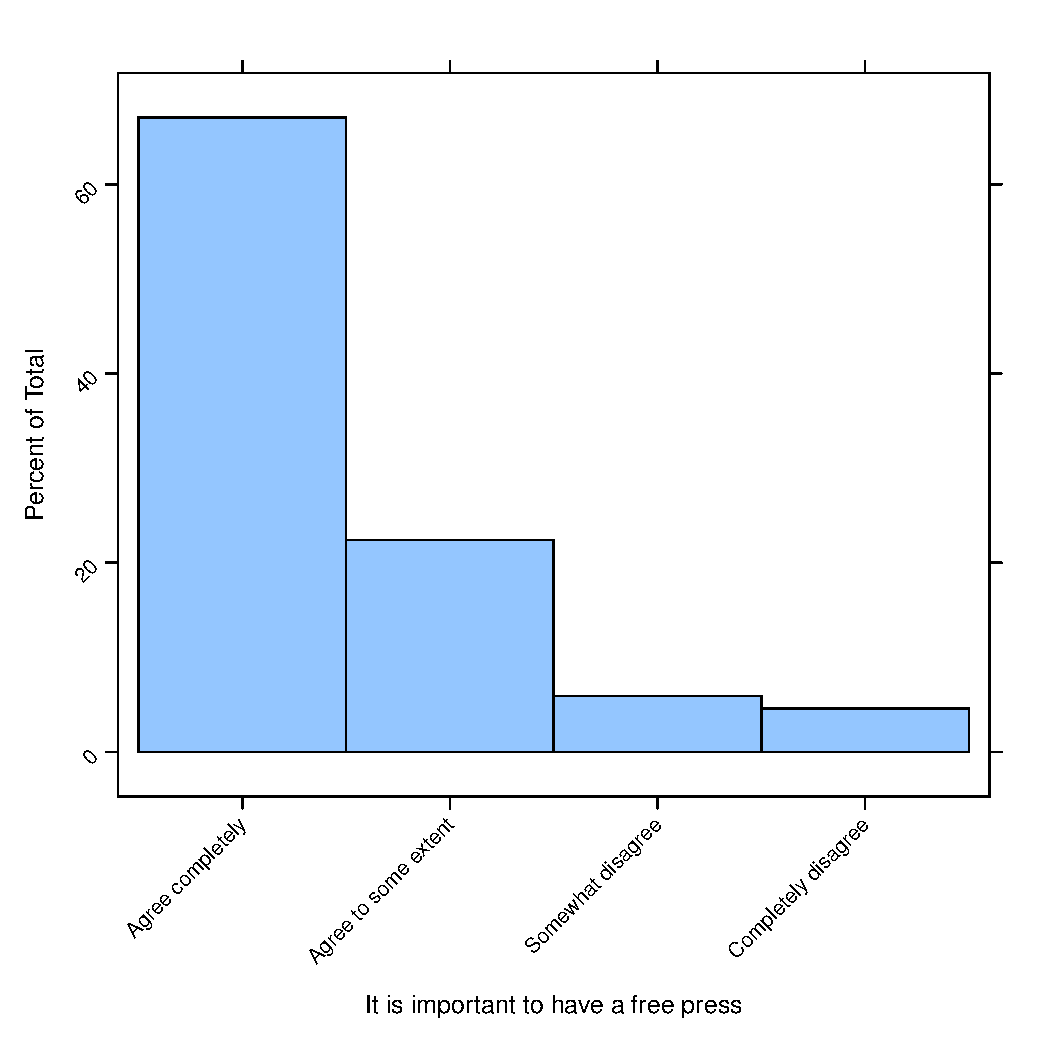
\includegraphics[scale=0.35, center]{/Users/hectorbahamonde/research/democratic_backsliding/free_press.pdf}
\end{center}
\end{frame}



\section{Discussion}

\subsection{Wrapping Up}

\miniframeson
\begin{frame}[c]{Main Takeaways: More Questions Than Answers}
  \begin{itemize}
    \item Hipotetizamos que los \emph{electoral losers} estarian mas dispuestos a apoyar acciones no-democraticas (protestas anti-sistemicas).
    \item Registramos esta hipotesis.
    \item Sin embargo, no encontramos resultados que van en linea con nuestras expectativas iniciales.
    \item {\color{red}Preguntas para ustedes}: {\bf cometimos un error en mezclar a la derecha con ``protestas''?}
  \end{itemize}
\end{frame}

\miniframesoff
\begin{frame}[c]{Thank you}
        \begin{center}
          \vspace{-0.7cm}\includegraphics[scale=.06, center]{/Users/hectorbahamonde/hbahamonde.github.io/resources/qr-code.pdf}
        \end{center}


        \begin{itemize}
            %\item Paper (draft) available at {\color{blue}www.HectorBahamonde.com}.
            \item[] {\large\color{red}\faCamera}\; to check updates on this project. 
        \end{itemize}
\end{frame}


%%%%%%%%%%%%%%%%%%%%%%%%%%%%%%%%
% APPENDIX
%%%%%%%%%%%%%%%%%%%%%%%%%%%%%%%%

\section{Appendix}

\subsection{Sum stats}

\miniframeson
\begin{frame}[shrink=5, plain]{\hypertarget{sum:table:slide}{{\tiny Summary Stats}}}

\begin{table}[!htbp] \centering \renewcommand*{\arraystretch}{1.1}\caption{Summary Statistics}\resizebox{\textwidth}{!}{
\begin{tabular}{lrr}
\hline
\hline
Variable & N & Percent \\ 
\hline
Age & 741 &  \\ 
... 18-24 & 120 & 16\% \\ 
... 25-34 & 172 & 23\% \\ 
... 35-44 & 146 & 20\% \\ 
... 45-54 & 146 & 20\% \\ 
... M<c3><a1>s de 55 & 157 & 21\% \\ 
Gender & 741 &  \\ 
... Man & 315 & 43\% \\ 
... Woman & 422 & 57\% \\ 
... Otro/Prefiero no decir & 4 & 1\% \\ 
Education & 741 &  \\ 
... Educaci<c3><b3>n b<c3><a1>sica completa (hasta octavo b<c3><a1>sico). & 10 & 1\% \\ 
... Educaci<c3><b3>n media completa. & 192 & 26\% \\ 
... Educaci<c3><b3>n t<c3><a9>cnico-profesional completa. & 214 & 29\% \\ 
... Educaci<c3><b3>n universitaria completa. & 270 & 36\% \\ 
... Magister o Doctorado completo. & 42 & 6\% \\ 
... Menos que educaci<c3><b3>n b<c3><a1>sica (menos que octavo b<c3><a1>sico). & 2 & 0\% \\ 
... Otro/Prefiero no decir & 11 & 1\% \\ 
Income & 741 &  \\ 
... De \$1000.001 a \$2.000.000 mensuales liquidos & 155 & 21\% \\ 
... De \$110.001 a \$150.000 mensuales liquidos  & 7 & 1\% \\ 
... De \$150.001 a \$225.000 mensuales liquidos & 20 & 3\% \\ 
... De \$2.000.001 a \$3.000.000 mensuales liquidos & 48 & 6\% \\ 
... De \$225.001 a \$350.000 mensuales liquidos & 35 & 5\% \\ 
... De \$3.000.001 a \$4.500.000 mensuales liquidos & 31 & 4\% \\ 
... De \$35.001 a \$75.000 mensuales liquidos & 14 & 2\% \\ 
... De \$350.001 a \$450.000 mensuales liquidos  & 48 & 6\% \\ 
... De \$450.001 a \$550.000 mensuales liquidos & 68 & 9\% \\ 
... De \$550.001 a \$700.000 mensuales liquidos & 86 & 12\% \\ 
... De \$700.001 a \$1.000.000 mensuales liquidos & 146 & 20\% \\ 
... De \$75.001 a \$110.000 mensuales liquidos & 18 & 2\% \\ 
... Menos de \$35.000 mensuales liquidos & 28 & 4\% \\ 
... M<c3><a1>s de \$4.500.000 mensuales liquidos & 16 & 2\% \\ 
... No sabe / No contesta & 21 & 3\%\\ 
\hline
\hline
\end{tabular}
}
\end{table}



\end{frame}

\subsection{References}

\miniframeson
\begin{frame}[shrink=35]
\vspace{1cm}\printbibliography
\end{frame} 


\end{document}




                                                                                                                                                                               
